%%%%%%%%%%%%%%%%%%%%%%%%%%%%%%%%%%%%%%%%%%%%%%%%%%%%%%%%%%%%%%%
%
% Welcome to Overleaf --- just edit your LaTeX on the left,
% and we'll compile it for you on the right. If you open the
% 'Share' menu, you can invite other users to edit at the same
% time. See www.overleaf.com/learn for more info. Enjoy!
%
%%%%%%%%%%%%%%%%%%%%%%%%%%%%%%%%%%%%%%%%%%%%%%%%%%%%%%%%%%%%%%%
\documentclass[unicode,11pt]{beamer}
\usetheme{Madrid}
\usepackage{listings}
\definecolor{links}{HTML}{2A1B81}
\hypersetup{colorlinks,linkcolor=,urlcolor=links}

\title{Scientific Computing on AWS}
\subtitle{Lecture 4: Serverless Computing}
\author{Tomoyuki Mano}
\institute[OIST]{Okinawa Institute of Science and Technology}
\date{2021/10/01 @OIST}

\begin{document}

\frame{\titlepage}

\begin{frame}{Lecture materials}
\begin{itemize}
    \item The main lecture material is at
    \url{https://tomomano.github.io/learn-aws-by-coding/en/}
    (sorry, I still haven't finished it all)
    \item The source code for the exercises is at
    \url{https://github.com/tomomano/learn-aws-by-coding}
    \item Supporting lecture slides are posted at
    \url{https://github.com/tomomano/oist-aws-2021}
\end{itemize}
\end{frame}

\begin{frame}{Course details}
\centering
\url{https://groups.oist.jp/grad/mini-course-2}

\vspace{10pt}

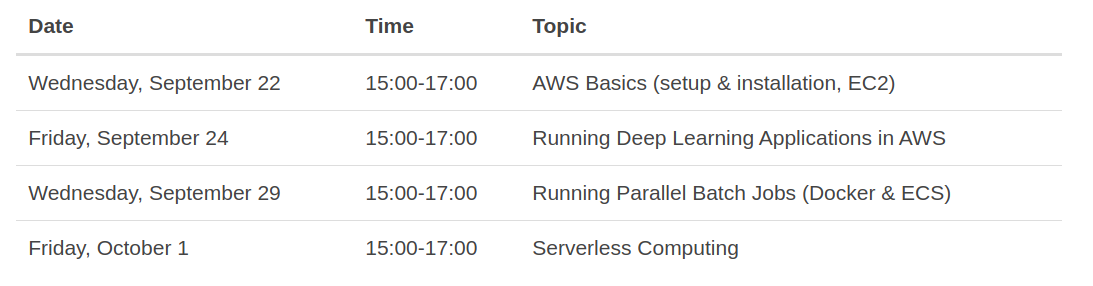
\includegraphics[width=1.0\textwidth]{imgs/schedule.png}

\begin{itemize}
    \item We will work on hands-on tutorial in all lectures, using real AWS cloud
    \item Let's make this interactive! Interrupt me anytime when you have questions.
\end{itemize}
\end{frame}

\begin{frame}{AWS Educate Program}

\begin{itemize}
    \item AWS Educate program generously gave us \$500 credit to use on AWS
    \item The credit was deposited on my personal AWS account.
    I created a child account for each student (see next slide).
    For the course exercises, please use this account, not your personal AWS account.
    \item We are sharing the \$500 credit with the entire class.
    Please do not overuse it, otherwise we run out of the credit!
    If I observe an individual using too much AWS credit, I will need to terminate that account.
    \item Accounts issued for you are valid until the end of this course (10/01).
\end{itemize}
\end{frame}

\begin{frame}{AWS Account}

\begin{itemize}
    \item I sent each student an invitation to AWS
    \item With this invitation, your account will be created under the "organization".
    Essentially, all the billing will go to the organization, not to you!
    \item \textbf{Once the invitation is sent to you, go to the login window, type your OIST email as account name, and click "reset password".}
    \item If you already have an AWS account created with OIST email, you can continue using that account.
    However, all cloud cost will be billed to the organization, not to you.
    If your account does anything other than the course exercise, please let me know.
\end{itemize}

\end{frame}

\end{document}

